\begin{TP} [Le lièvre et la tortue][\tice \algo]

\partie{Première course}
Une partie du jeu du lièvre et de la tortue se déroule de la façon suivante:\\
\parbox{0.8\linewidth}{
\begin{cadre}[H1][H4]
La distance à parcourir est de 6 cases.
\begin{itemize}
\item On lance un dé.
\item Si on obtient 6, le lièvre avance de 6 cases.
\item Sinon, la tortue avance d'une case.
\end{itemize}
\end{cadre}}\\
%\vspace{-1.5em}
\begin{enumerate}
\item \`A priori, qui a le plus de chances de gagner?
\item Faire une simulation à l'aide d'un tableur ou d'un algorithme.\\
Donner une valeur approchée de la probabilité que le lièvre gagne.
\item \`A l'aide d'un arbre, calculer la probabilité que la tortue gagne. \\
En déduire la probabilité que le lièvre gagne.
\end{enumerate}

\partie{Deuxième course}
Les règles changent!\\
\parbox{0.8\linewidth}{
\begin{cadre}[J1][J4]

\begin{itemize}
\item La distance a parcourir est maintenant de 4 cases.
%\item La tortue a mangé une super salade:\\ elle effectue la course en 4 cases.
\item Le lièvre a mangé une super carotte:\\ il avance de 4 cases quand on obtient 5 ou 6 au lancer de dé.
\end{itemize}
\end{cadre}}\\
\vspace{-1.5em}

\begin{enumerate}
\item Adapter la simulation à cette situation.\\Donner une approximation de la nouvelle loi de probabilité.
\item \`A l'aide de l'arbre, retrouver la distribution de probabilité.
\end{enumerate}
\end{TP}

\begin{TP}[Full]
Le jeu de yams se joue avec 5 dés. On essaye de faire des combinaisons diverses et on a le droit de relancer deux fois tout ou une partie des dés.\\
Corinne a obtenu au 1\ier\~lancer trois 4, un 2 et un 5. Elle voudrait faire un full (3 dés d'une valeur et 2 dés d'une autre). Elle hésite entre garder les trois 4 et le 5 et relancer le  dé indiquant 2 ou garder les trois 4 et relancer les deux autres dés. Aide-la à résoudre ce dilemme.

\vspace{1cm}
\begin{center}
 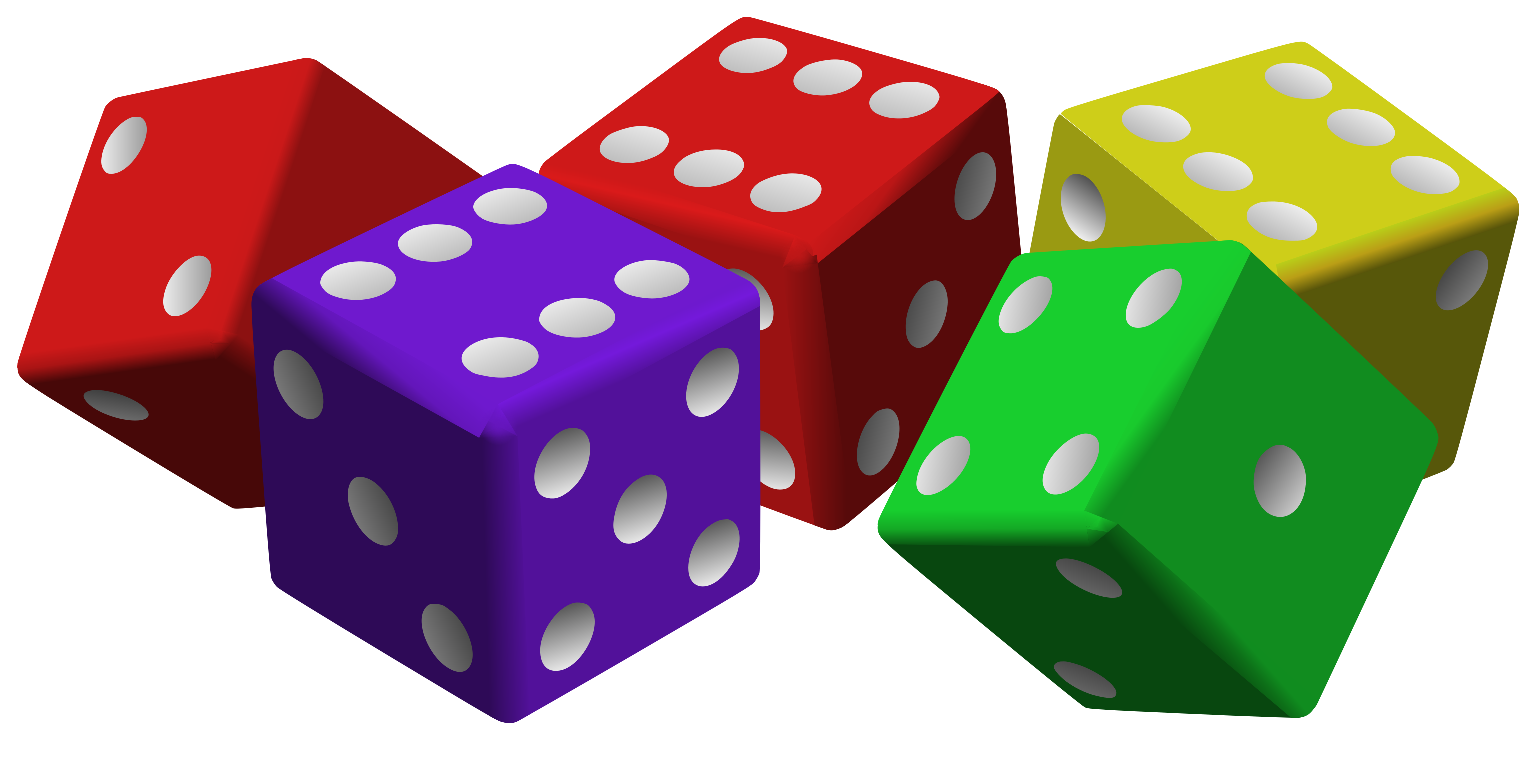
\includegraphics[width=6cm]{./2SP3/images/Five_dice_02.eps}
 % Five_dice_02.eps: 0x0 pixel, 300dpi, 0.00x0.00 cm, bb=
\end{center}

\end{TP}

\clearpage
\begin{TP}[Algorithme de Monte-Carlo][ \tice]
%\vspace{-1.5em}
\begin{enumerate}
\item Dans un repère orthonormé $(O; I, J)$, on considère un disque de centre $O$ et de rayon 1 et un carré de centre $O$ et de côté 2 comme sur le graphique ci-dessous.
	\begin{enumerate}
	\item Déterminer l'aire du disque et l'aire du carré.
	\item Quelles conditions doivent vérifier les coordonnées d'un point $M$ pour qu'il soit à l'intérieur du carré?
	\item Quelles conditions doivent vérifier les coordonnées de $M$ pour que $OM\leqslant 1$ ? \\
	Dans ce cas, que peut-on en déduire pour $M$ ?

\begin{center}
\begin{tikzpicture}[general]
\draw [quadrillage] (-1.55,-1.46) grid (1.71,1.48);
\draw[color=A1,fill=A4] (-1,1) -- (-1,-1) -- (1,-1) -- (1,1) -- cycle;
\draw[->,color=black] (-1.55,0) -- (1.71,0);
\draw[->,color=black] (0,-1.46) -- (0,1.48);
\draw (1,0) node[below right] {1};
\draw (0,1) node[above left] {1};
\draw (-1,0) node[below left] {$-1$};
\draw (0,-1) node[below left] {$-1$};
\draw (0,0) node[below left] {0};
\draw(0,0) circle (1cm);
\draw [color=A1] (-1,1)-- (-1,-1);
\draw [color=A1] (-1,-1)-- (1,-1);
\draw [color=A1] (1,-1)-- (1,1);
\draw [color=A1] (1,1)-- (-1,1);
\end{tikzpicture}
\end{center}
	\end{enumerate}
	\vspace{-1.5em}
\item L'algorithme de Monte-Carlo calcule une valeur approchée de $\pi$ en créant un grand nombre de points aléatoires dans le carré, et en observant combien se trouvent dans le disque. Le rapport du nombre de points dans le disque sur le nombre total de points devrait être proche du rapport de l'aire du disque sur l'aire du carré et nous permettra de calculer $\pi$.
	\begin{enumerate}
	\item Complète l'algorithme ci-dessous.
	{\small
 \begin{center}
\begin{algorithme}
\titreAlgo{algorithme mystère}
\BLOCKvariables
\DeclareVar{x,y,pi}{nombre réel}{}
%\DeclareVar{y}{nombre réel}{}
\DeclareVar{k, n, compteur}{nombre entier}{}
%\DeclareVar{n}{nombre entier}{}
%\DeclareVar{compteur}{nombre entier}{}
%\DeclareVar{pi}{nombre réel}{}
\BLOCKtraitements
\Demander{n}
\DonnerValeur{compteur}{0}
\pour{k}{1}{n}{
\DonnerValeur{x}{un nombre aléatoire entre \dots et \dots}
\DonnerValeur{y}{un nombre aléatoire entre \dots et \dots}
\sialors{\dots}{
\DonnerValeur{compteur}{compteur+1}}}
 \DonnerValeur{pi}{compteur/n}
\DonnerValeur{pi}{pi $\times$ \dots}
\BLOCKaffichage
\Afficher{\og $\pi$ vaut environ : \fg}
\AfficherVar{pi}
\finAlgo
        \end{algorithme}
\end{center}}
	\item Implémenter cet algorithme sur un ordinateur ou sur une calculatrice.\\
	 Le tester avec différentes valeurs de $n$.
	\item Trouve-t-on toujours la même valeur approchée pour $\pi$?
	\end{enumerate}
\item Paul affirme qu'on peut connaître la précision de notre valeur approchée de $\pi$. A-t-il raison?
\end{enumerate}

\end{TP}




\begin{TP}[Problème de Monty Hall] [\tice]
Sur le plateau d'un jeu télévisé, il y a trois portes dont une cache une
voiture et les deux autres une chèvre. Il s'agit de choisir une des portes pour gagner ce qu'il y a derrière.

Le jeu se déroule en 3 étapes:
\begin{itemize}
\item le joueur choisit une porte mais ne l'ouvre pas;
\item l'animateur, qui sait où se trouve la voiture, ouvre une autre porte que celle choisie et qui cache une chèvre;
\item l'animateur propose au joueur de changer son choix initial.
\end{itemize}
Le joueur a-t-il intérêt à modifier son choix?
\begin{enumerate}
\item L'algorithme ci-dessous permet de faire une simulation de ce
problème.\\ Compléter-le puis effectuer la simulation.
%{\footnotesize 
\begin{center}
\begin{algorithme}
\titreAlgo{Problème de Monty Hall}
\BLOCKvariables
\DeclareVar{NbEssais}{nombre entier}{}
\DeclareVar{Change}{nombre réel}{}
\DeclareVar{NeChangePas}{nombre réel}{}
\DeclareVar{PorteGagnante}{nombre entier}{}
\DeclareVar{PorteChoisie}{nombre entier}{}
\DeclareVar{k}{nombre entier}{}
\BLOCKtraitements
\Demander{NbEssais}
\DonnerValeur{Change}{0}
\DonnerValeur{NeChangePas}{0}
\pour{k}{1}{NbEssais}{
    \DonnerValeur{PorteGagnante}{un nombre aléatoire entre 1 et 3}
    \DonnerValeur{PorteChoisie}{un nombre aléatoire entre 1 et 3}
    \sialorssinon{PorteChoisie =PorteGagnante}{
        \DonnerValeur{\dots}{\dots+1}}{
        \DonnerValeur{\dots}{\dots+1}}
    }
\DonnerValeur{Change}{Change/NbEssais}
\DonnerValeur{NeChangePas}{NeChangePas/NbEssais}
\BLOCKaffichage
\Afficher{\og La probabilité de gagner en changeant est de \fg}
\AfficherVar{Change}
\Afficher{\og La probabilité de gagner en ne changeant pas est de \fg}
\AfficherVar{NeChangePas}
\finAlgo
\end{algorithme}
\end{center}
\item Que peut-on en conclure?
\item Que se passe-t-il si on joue maintenant avec quatre portes dont une
seule gagnante?
\end{enumerate}

\end{TP}



